\section{Roadmap au 08/01/2022}

\subsection{Éléments de la roadmap}

Une des premières versions de la roadmap, après la phase de pré-developpement et la session de 
plannification du premier sprint est la suivante. Comme mentionné, cette roadmap a vecu au cours 
du projet, et une roadmap mise à jour pour chaque sprint est présentée plus loin pour chacun des 
sprints.

\noindent%
\includegraphics[scale=0.5]{images/roadmap_prepa.png}

\noindent%
\includegraphics[scale=0.45]{images/roadmap_alpha.png}\\
\includegraphics[scale=0.45]{images/roadmap_beta.png}\\
\includegraphics[scale=0.45]{images/roadmap_RC.png}\\
\includegraphics[scale=0.45]{images/roadmap_prod.png}

\newpage
\subsection{Gantt (version initiale)}

Voici le diagramme Gantt complet édité en janvier 2022. Comme la roadmap il a évolué au fil du temps
 et une version mise a jour pour chaque sprint est présentée plus loin.

\noindent%
\begin{center}
    \includegraphics[scale=0.5]{images/Gantt_prepa.png}
\end{center}

\newpage
\subsection{Gantt (dernière version)}

Voici la dernière version du Gantt après modifications au cours du projet.

\noindent%
\begin{center}
    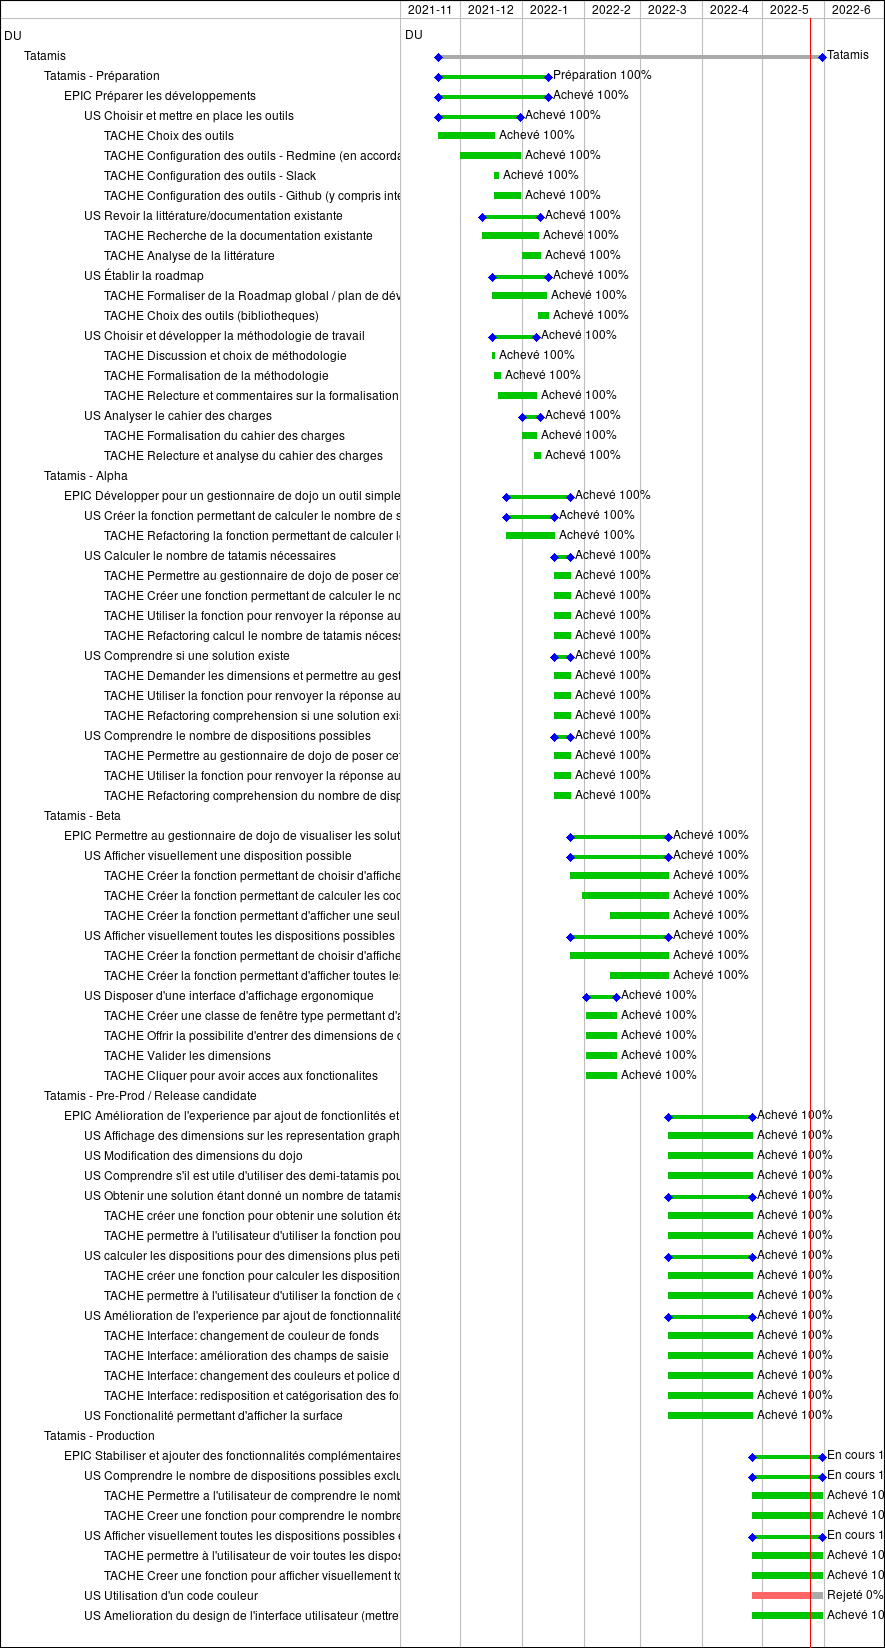
\includegraphics[height=21.5cm]{images/Gantt_final.png}
\end{center}